\section{Conclusion}

We presented CSI-to-language conversion as a grounded inference problem rather than open-ended
generation. CSI2TEXT-PGMT first recovers a typed channel state using configuration-aware,
target-specific physical representations and then converts the corrected record into an auditable
description through deterministic verbalization. The resulting reports are structurally complete and
substantially more accurate than direct learned decoders on the underlying numerical quantities. The
generalization, split-sensitivity, and observation-noise studies further show that the decisive challenge
is not fluent language generation, but the recovery of indirect multipath structure, especially under
NLoS propagation. This factorization provides an interpretable interface for wireless-channel
analytics while making both successes and failures traceable to explicit physical fields. Future work
should extend the framework to measured channels, hardware impairments, calibrated uncertainty, and
more expressive multipath-aware objectives.

\begin{thebibliography}{99}

\bibitem{alkhateeb2019deepmimo}
Ahmed Alkhateeb. DeepMIMO: A generic deep learning dataset for millimeter wave and massive
MIMO applications. \emph{arXiv preprint arXiv:1902.06435}, 2019.

\bibitem{chen2018gradnorm}
Zhao Chen, Vijay Badrinarayanan, Chen-Yu Lee, and Andrew Rabinovich. GradNorm: Gradient
normalization for adaptive loss balancing in deep multitask networks. In \emph{Proceedings of the
35th International Conference on Machine Learning}, volume 80, pages 794--803, 2018.

\bibitem{deepseek2025r1}
DeepSeek-AI. DeepSeek-R1: Incentivizing reasoning capability in LLMs via reinforcement learning.
\emph{arXiv preprint arXiv:2501.12948}, 2025.

\bibitem{ferrand2023charting}
Paul Ferrand, Maxime Guillaud, Christoph Studer, and Olav Tirkkonen. Wireless channel charting:
Theory, practice, and applications. \emph{arXiv preprint arXiv:2304.08095}, 2023.

\bibitem{fleury1999sage}
Bernard H. Fleury, Martin Tschudin, Rainer Heddergott, Dirk Dahlhaus, and Klaus I. Pedersen.
Channel parameter estimation in mobile radio environments using the SAGE algorithm. \emph{IEEE
Journal on Selected Areas in Communications}, 17(3):434--450, 1999.

\bibitem{guo2017calibration}
Chuan Guo, Geoff Pleiss, Yu Sun, and Kilian Q. Weinberger. On calibration of modern neural
networks. In \emph{Proceedings of the 34th International Conference on Machine Learning},
volume 70, pages 1321--1330, 2017.

\bibitem{internlm2025}
InternLM Team. InternLM3-8B-Instruct Model Card. Hugging Face model repository, 2025.
\url{https://huggingface.co/internlm/internlm3-8b-instruct}.

\bibitem{keya2026wirelesssense}
Mahmuda Keya, Sneh Pillai, Jiawei Yuan, Kai Zeng, and Long Jiao. WirelessSenseLLM: Zero-shot
human activity understanding by bridging wireless signals and human language. \emph{arXiv preprint
arXiv:2605.14070}, 2026.

\bibitem{liu2024wifo}
Boxun Liu, Shijian Gao, Xuanyu Liu, Xiang Cheng, and Liuqing Yang. WiFo: Wireless foundation
model for channel prediction. \emph{arXiv preprint arXiv:2412.08908}, 2024.

\bibitem{orekondy2023winert}
Tribhuvanesh Orekondy, Pratik Kumar, Shreya Kadambi, Hao Ye, Joseph Soriaga, and Arash
Behboodi. WiNeRT: Towards neural ray tracing for wireless channel modelling and differentiable
simulations. In \emph{International Conference on Learning Representations}, 2023.

\bibitem{palhares2025csi2vec}
Victoria Palhares, Sueda Taner, and Christoph Studer. CSI2Vec: Towards a universal CSI feature
representation for positioning and channel charting. \emph{arXiv preprint arXiv:2506.05237}, 2025.

\bibitem{qwen2025}
Qwen Team. Qwen3 Technical Report. \emph{arXiv preprint arXiv:2505.09388}, 2025.

\bibitem{qwen2026}
Qwen Team. Qwen3.5-2B Model Card. Hugging Face model repository, 2026.
\url{https://huggingface.co/Qwen/Qwen3.5-2B}.

\bibitem{radford2021clip}
Alec Radford, Jong Wook Kim, Chris Hallacy, Aditya Ramesh, Gabriel Goh, Sandhini Agarwal,
Girish Sastry, Amanda Askell, Pamela Mishkin, Jack Clark, Gretchen Krueger, and Ilya Sutskever.
Learning transferable visual models from natural language supervision. In \emph{Proceedings of the
38th International Conference on Machine Learning}, volume 139, pages 8748--8763, 2021.

\bibitem{roy1989esprit}
Richard Roy and Thomas Kailath. ESPRIT-estimation of signal parameters via rotational invariance
techniques. \emph{IEEE Transactions on Acoustics, Speech, and Signal Processing},
37(7):984--995, 1989.

\bibitem{schmidt1986music}
Ralph O. Schmidt. Multiple emitter location and signal parameter estimation. \emph{IEEE
Transactions on Antennas and Propagation}, 34(3):276--280, 1986.

\bibitem{scholak2021picard}
Torsten Scholak, Nathan Schucher, and Dzmitry Bahdanau. PICARD: Parsing incrementally for
constrained auto-regressive decoding from language models. In \emph{Proceedings of the 2021
Conference on Empirical Methods in Natural Language Processing}, pages 9895--9901, 2021.

\bibitem{studer2018charting}
Christoph Studer, Said Medjkouh, Emre Gonultas, Tom Goldstein, and Olav Tirkkonen. Channel
charting: Locating users within the radio environment using channel state information. \emph{IEEE
Access}, 6:47682--47698, 2018.

\bibitem{rayverse2025}
UNIC Lab. RayVerse: A large-scale urban radio-propagation dataset generated using ray tracing,
2025. \url{https://github.com/UNIC-Lab/RayVerse}. Accessed July 27, 2026.

\bibitem{wei2026wifi2cap}
Tzu-Ti Wei, Chu-Yu Huang, Yu-Chee Tseng, and Jen-Jee Chen. WiFi2Cap: Semantic action
captioning from Wi-Fi CSI via limb-level semantic alignment. \emph{arXiv preprint
arXiv:2603.22690}, 2026.

\bibitem{wiworldrealdata}
Wi-World. \emph{RealData Dataset README\_Chinese}. Official dataset documentation.

\bibitem{zhu2024physics}
Guangxu Zhu, Yuanming Sun, and Kaibin Ji. Physics-informed generalizable wireless channel
modeling with segmentation and deep learning: Fundamentals, methodologies, and challenges.
\emph{arXiv preprint arXiv:2401.01288}, 2024.

\bibitem{zou2026rfgpt}
Hang Zou, Yu Tian, Bohao Wang, Lina Bariah, Samson Lasaulce, Chongwen Huang, and Merouane
Debbah. RF-GPT: Teaching AI to see the wireless world. \emph{arXiv preprint
arXiv:2602.14833}, 2026.

\end{thebibliography}

\clearpage
\appendices

\section{Target Construction and Physical Scope}

This appendix defines the simulator-derived quantities represented by the structured record. These
definitions establish annotation semantics and reproducibility; they are not additional learned
components.

\subsection{Valid Paths, First Path, and Absolute Power}

Let $\mathcal P$ be the finite set of paths retained by the D2Los/RayVerse export:
\[
\mathcal P=\{p\mid P_p^{\mathrm{dBW}}\ \text{and}\ \tau_p\ \text{are finite}\}.
\]
No additional relative-power threshold is applied. The first path is the earliest retained path,
\[
p^\star=\arg\min_{p\in\mathcal P}\tau_p,
\qquad
\tau_1=\tau_{p^\star},
\qquad
p_1^{\mathrm{dBW}}=P_{p^\star}^{\mathrm{dBW}}.
\]
Simulator path loss $L_p^{\mathrm{dB}}$ is converted to received-path power using the fixed transmit
power $P_{\mathrm{tx}}=23$ dBm:
\[
P_p^{\mathrm{dBW}}=P_{\mathrm{tx}}^{\mathrm{dBm}}-L_p^{\mathrm{dB}}-30.
\]
The first-path-power target is therefore an absolute value under this transmit-power assumption, not
a per-link relative value. This definition motivates the raw-scale bypass in the model: per-example
standardization benefits representation learning but removes the amplitude scale required by the power
head.

\subsection{Delay Spread, Angular Spread, and the K-Factor Label}

With linear power $P_p=10^{P_p^{\mathrm{dBW}}/10}$, the delay-spread label is the power-weighted
RMS spread,
\[
\bar\tau=\frac{\sum_pP_p\tau_p}{\sum_pP_p},
\qquad
\sigma_\tau=\sqrt{\frac{\sum_pP_p(\tau_p-\bar\tau)^2}{\sum_pP_p}}.
\]
Angular spread uses circular statistics. With $w_p=P_p/\sum_qP_q$,
\[
R=\left|\sum_pw_pe^{j\theta_p}\right|,
\qquad
\sigma_\theta=\frac{180}{\pi}\sqrt{-2\log(\operatorname{clip}(R,10^{-6},1))}.
\]
For a LoS link with residual reflected paths, the simulator-derived ray-power-ratio label is
\[
K_{\mathrm{dB}}=10\log_{10}\frac{P_0}{\sum_{p\geq1}P_p}.
\]
NLoS links are assigned $-20$ dB, and a LoS link with no residual path is assigned 30 dB. This is
a derived label based on the retained ray powers, not a multi-snapshot Rician $K$ estimator.

\subsection{Path and Reflection-Interaction Semantics}

The supplied CSI dataset contains reflected propagation paths and does not include diffraction or
scattering components. Consequently, the stored interaction counts can be interpreted as reflection
interactions for this dataset. Let $c_p$ be the stored reflection-interaction count of retained path $p$.
The record distinguishes
\[
n_{\mathrm{refl}}=\sum_{p\in\mathcal P}\min(c_p,9),
\qquad
n_{\mathrm{rpath}}=\sum_{p\in\mathcal P}\mathbf 1[c_p>0],
\]
where $n_{\mathrm{refl}}$ is the total encoded reflection-interaction count and
$n_{\mathrm{rpath}}$ is the number of reflected paths. A single path may contain multiple reflections,
so these quantities are related but not identical. Path count is read from the export without a new
top-$K$ truncation. An audit of 742,818 links from 20 source files found one to five saved paths per
link; five is an empirical ceiling of the supplied exports, not a universal physical limit.

\subsection{Observability Boundaries}

The retained spatial aperture is on the transmitter side and only one receive element is supplied.
Frequency-dependent phase supports delay inference, and the transmitter array supports
transmitter-side spatial structure. Receiver-side AoA is therefore treated as a supervised
cross-domain target learned from correlations among transmitter-side beam-frequency CSI, multipath
structure, and ray-traced geometry. It must not be interpreted as a directly measured receive-array
beam direction. For the same reason, classical receive-array estimators such as MUSIC, ESPRIT, and
Bartlett are not commensurate baselines for the receiver-side angle labels in this dataset.

\section{Implementation and Evaluation Details}

\subsection{Encoder, Alignment, and Prediction Heads}

ULA inputs use an antenna-axis FFT and group four adjacent beams per token. UPA inputs use a
row-column two-dimensional FFT and $2\times2$ local beam patches. Real and imaginary components
are concatenated. The shared encoder combines a linear frequency projection, depthwise-pointwise
convolution, adaptive average/max summaries, feature-wise configuration modulation, beam-position
embeddings, and carrier/frequency encodings.

The Transformer has six layers, hidden width 384, six attention heads, and a 1,536-dimensional
feed-forward block. The fused $[\mathrm{CLS}]$ and masked-mean representation is projected to a
normalized 256-dimensional CSI embedding. Descriptions use a 300-token vocabulary with maximum
length 48. A three-layer, four-head Transformer of width 256 produces the text embedding. Semantic
prototype keys combine environment, LoS/NLoS status, path richness, delay and angular regimes,
$K$ bin, and reflection statistics; classes with fewer than five training samples are discarded.

For completeness, the alignment loss retains the full symmetric pairwise InfoNCE form used in the
initial draft. For two normalized embedding families $z_a$ and $z_b$ in a minibatch of size $N$,
\begin{align}
\mathcal L_{a,b}=-\frac{1}{2N}\sum_{i=1}^{N}\bigg[&
\log\frac{\exp\!\left((z_a^i)^\top z_b^i/T\right)}
{\sum_{j=1}^{N}\exp\!\left((z_a^i)^\top z_b^j/T\right)} \notag\\[-2pt]
&+\log\frac{\exp\!\left((z_b^i)^\top z_a^i/T\right)}
{\sum_{j=1}^{N}\exp\!\left((z_b^i)^\top z_a^j/T\right)}\bigg].
\label{eq:symmetric-infonce}
\end{align}
The initial temperature is $T=0.07$. Equation~\ref{eq:symmetric-infonce} is instantiated for
CSI--text, CSI--prototype, and text--prototype pairs. Thus both retrieval directions contribute to
each pairwise term rather than treating one embedding family as a fixed one-way target.

Temporal quantities use frequency- and delay-domain features, angular quantities use circular
representations, and absolute power combines the standardized representation with the raw-scale
bypass. Reflection-interaction count and reflected-path count use separate prediction heads because
one path may contain multiple reflection interactions.

\subsection{Loss Weights and Optimization}

\begin{table}[t]
\centering
\caption{Loss configuration used for the main model.}
\label{tab:appendix-loss}
\scriptsize
\setlength{\tabcolsep}{2pt}
\resizebox{\columnwidth}{!}{%
\begin{tabular}{lcc}
\toprule
Group & Term & Weight \\
\midrule
Alignment & CSI--text / CSI--prototype / text--prototype & 1.0 / 1.0 / 1.0 \\
Representation & semantic / attribute / auxiliary physics & 0.5 / 0.1 / 0.005 \\
$K$ factor & strong-bin classifier / within-bin position & 0.5 / 0.1 \\
First delay & normalized / raw / fused raw & 0.08 / 0.001 / 0.02 \\
First delay & bin / position / consistency / tail underestimate & 0.02 / 0.01 / 0.01 / 0.01 \\
Delay spread & raw / bin / within-bin position & 0.0005 / 0.03 / 0.008 \\
LoS delay & regression / nonnegative / consistency & 0.05 / 0.005 / 0.005 \\
Angles & LoS / first path / NLoS first path & 0.05 / 0.02 / 0.01 \\
First power & bin / position; NLoS multiplier & 0.03 / 0.1; 2.0 \\
Reflections & classifier / regression; NLoS multiplier & 0.02 / 0.01; 1.0 \\
\bottomrule
\end{tabular}}
\end{table}

Table~\ref{tab:appendix-loss} records the main loss configuration. The optional relational training
regularizer has weight zero in the reported main runs; record-level correction is applied after
prediction.

Models train for 100 epochs with AdamW, batch size 128, initial learning rate $3\times10^{-4}$,
weight decay $10^{-2}$, five epochs of linear warm-up, and cosine decay to $10^{-5}$. Every epoch
traverses all 40,000 main training examples. Retaining the final incomplete minibatch gives 313
minibatches per epoch and 31,300 scheduled optimizer steps. Unless stated otherwise, seeds are 0, 1,
and 2, and error bars are sample standard deviations. The balanced main model has 28,938,178
trainable parameters. A run uses one NVIDIA RTX 4090 with 23.6 GB memory, PyTorch 2.5.1 with
CUDA 12.1, and no automatic mixed precision; a representative run takes approximately 5.5 hours.

\subsection{Data Cohorts and Split Construction}

\begin{table*}[t]
\centering
\caption{Core cohorts and isolation rules.}
\label{tab:cohort-core}
\scriptsize
\setlength{\tabcolsep}{4pt}
\begin{tabular}{lccc>{\centering\arraybackslash}p{5.2cm}}
\toprule
Cohort & Purpose & Train/test & LoS/NLoS & Isolation and use \\
\midrule
SRC-400K & source pool & 400K & original & no train/test split; source for subsequent sampling \\
MAIN-50K-v1 & main experiment & 40K/10K & 20K/20K; 5K/5K & 78 training and 19 test maps with zero group-ID overlap; full model, conventional baselines, and architectural ablations \\
SD-50K & scenario isolation & 40K/10K & balanced & map-, spatial-block-, UE-position-, and group-disjoint scenario evaluation \\
\bottomrule
\end{tabular}
\end{table*}

\begin{table*}[t]
\centering
\caption{Specialized cohorts. Reflection labels are available unless otherwise noted.}
\label{tab:cohort-specialized}
\scriptsize
\setlength{\tabcolsep}{3.5pt}
\begin{tabular}{lccc>{\centering\arraybackslash}p{4.5cm}}
\toprule
Cohort & Purpose & Train/test & Balance & Isolation or label status \\
\midrule
CORR-100K & relational correction & 80K/20K & balanced & zero shared links/samples; 97 shared maps \\
RPATH-100K & reflected-path extension & 80K/20K & 13,628/86,372 & random split; map/link isolation not audited; reflected-path labels reconstructed and verified \\
DD-100K-v2 & decoder training & 40K/1K & balanced & zero shared links/samples; 97 shared maps; reconstructed labels \\
COST-50K-RPATH-v2 & cost benchmark & 40K/10K & balanced & zero shared links/samples; 97 shared maps \\
Noise-Augment-50K & noise study & 40K/10K & balanced & zero shared links/samples; 97 shared maps \\
\bottomrule
\end{tabular}
\end{table*}

All cohorts originate from the 400,000-link source pool. Tables~\ref{tab:cohort-core} and
\ref{tab:cohort-specialized} transcribe the cohort plan used across the main, stress-test, decoder,
correction, extension, and cost studies. Cohort-qualified names prevent numerical differences across
independently sampled experiments from being interpreted as contradictory estimates on one fixed
test set.

For complete map-disjoint evaluation, 78 of 97 source maps form a 321,644-example training parent
and 19 maps form a 78,356-example evaluation parent. Balanced subsets are sampled only within
their parents: 20,000 LoS and 20,000 NLoS links for training, and 5,000 of each for evaluation.
Ordered group IDs, maps, map-qualified spatial blocks, and exact UE positions are checked for empty
intersection. The spatial-block protocol has no guard band, so complete map separation remains the
stronger scenario-disjoint test.

The 400,000-link source pool contains 53,577 LoS and 346,423 NLoS examples. The exact test-map
IDs are
\begin{multline*}
\{1,7,15,17,21,22,25,28,30,34,\\
50,53,54,55,81,89,96,98,99\}.
\end{multline*}
all remaining map IDs are training-only. The balanced-subset samplers use seed 23,441 for training
and seed 23,442 for evaluation.

Split provenance is verified at four levels. First, the ordered training and evaluation group-ID lists
are compared directly. Second, each group is expanded to its map ID, map-qualified spatial-block ID,
and exact UE position, and every train--test intersection is required to be empty. Third, the ordered
10,000-example evaluation list stored with each run is compared with the audited evaluation manifest.
Fourth, each checkpoint record is bound to the exact training manifest and sampling seed used to fit
it. SHA-256 hashes of the complete ordered ID lists, rather than hashes of unordered sets or row counts,
are retained in the machine-readable audit. These checks detect three leakage failures that a row-count
or class-balance check cannot: (i) cohorts with the same LoS/NLoS balance but shared physical links,
(ii) different links sampled from a map that should have been held out in its entirety, and (iii) a
checkpoint trained from a manifest different from the one associated with the reported evaluation
table.

\subsection{Text Metrics and Tolerance Definitions}

\begin{table}[t]
\centering
\caption{Field-specific numerical tolerance accuracy on the balanced MAIN-50K-v1 evaluation split
(mean $\pm$ sample standard deviation over three seeds).}
\label{tab:field-tolerance-complete}
\scriptsize
\setlength{\tabcolsep}{3pt}
\begin{tabular}{lc}
\toprule
Field and tolerance & Accuracy $\uparrow$ \\
\midrule
Path count ($\pm1$) & $0.9533\pm0.0061$ \\
First-path delay ($\pm50$ ns) & $0.9451\pm0.0032$ \\
First-path angle ($\pm15^\circ$) & $0.6841\pm0.0102$ \\
First-path power ($\pm5$ dB) & $0.6436\pm0.0430$ \\
$K$ factor ($\pm3$ dB) & $0.7971\pm0.0302$ \\
Delay spread ($\pm50$ ns) & $0.9700\pm0.0003$ \\
Angular spread ($\pm15^\circ$) & $0.7907\pm0.0716$ \\
LoS delay ($\pm50$ ns) & $0.9915\pm0.0012$ \\
LoS angle ($\pm15^\circ$) & $0.9972\pm0.0007$ \\
Reflection-interaction count ($\pm1$) & $0.6562\pm0.0031$ \\
\bottomrule
\end{tabular}
\end{table}

Predicted and reference descriptions are parsed into typed slots. Categorical fields use accuracy and
macro-F1. Numeric-slot F1 measures whether required values are present. Hallucination is the fraction
of predicted numeric slots unsupported by the reference schema. Numerical tolerance accuracy checks
whether a present value is within 50 ns for delay, $15^\circ$ for angle, 5 dB for first-path power,
3 dB for $K$, and one count for path or reflection fields. Composite factuality is the macro average
of categorical accuracies, numeric-slot F1, numerical tolerance accuracy, and one minus hallucination.
It is not sentence exact match. Raw MAE remains necessary because the tolerance thresholds are
application choices.

The tolerance table complements MAE by exposing the fraction of fields that meet application-scale
error bands. It also shows why one aggregate numerical-accuracy value is insufficient: LoS-specific
geometry is highly reliable, whereas first-path power and reflection multiplicity remain harder.

\subsection{Baselines and Inference Settings}

Physics baselines include flattened CSI with an MLP, a CNN, PDP/IFFT features with an MLP, a
Transformer without specialized branches, and independent single-task heads on the same CSI
encoder. Direct learned decoders map the CSI encoder representation to a learned soft prefix for
Qwen3-1.7B, Qwen3.5-2B, InternLM3-8B, or DeepSeek-R1-Qwen3-8B. These decoders learn to emit
the same record schema but do not use the target-specific physical heads. The four decoder results are
single trained runs; their missing error bars must not be interpreted as zero variance.

\section{Additional Experimental Evidence}

This section adds protocols and evidence not already tabulated in the main paper. Main-text AWGN,
cross-configuration, split-sensitivity, propagation-regime, and language-alignment tables are not
repeated.

\subsection{Complete Main-Model Aggregate Performance}

\begin{table}[t]
\centering
\caption{Complete aggregate performance of CSI2TEXT-PGMT-MAIN-50K on the balanced main split
(mean $\pm$ sample standard deviation over three seeds).}
\label{tab:complete-main-fields}
\scriptsize
\setlength{\tabcolsep}{3pt}
\begin{tabular}{lc}
\toprule
Target & Result \\
\midrule
Environment accuracy (\%) $\uparrow$ & $100.00\pm0.00$ \\
LoS/NLoS accuracy (\%) $\uparrow$ & $99.58\pm0.11$ \\
Path-count MAE $\downarrow$ & $0.215\pm0.056$ \\
First-path delay MAE (ns) $\downarrow$ & $21.91\pm0.30$ \\
First-path angle MAE ($^\circ$) $\downarrow$ & $16.61\pm0.56$ \\
First-path power MAE (dB) $\downarrow$ & $4.34\pm0.27$ \\
$K$-factor MAE (dB) $\downarrow$ & $2.15\pm0.04$ \\
Delay-spread MAE (ns) $\downarrow$ & $11.30\pm0.26$ \\
Angular-spread MAE ($^\circ$) $\downarrow$ & $9.72\pm0.47$ \\
LoS-delay MAE (ns) $\downarrow$ & $8.83\pm0.55$ \\
LoS-angle MAE ($^\circ$) $\downarrow$ & $1.33\pm0.17$ \\
NLoS first-delay MAE (ns) $\downarrow$ & $40.66\pm1.58$ \\
NLoS first-angle MAE ($^\circ$) $\downarrow$ & $35.88\pm0.96$ \\
Reflection-interaction-count MAE $\downarrow$ & $1.032\pm0.019$ \\
Reflected-path-count MAE $\downarrow$ & $0.086\pm0.005$ \\
\bottomrule
\end{tabular}
\end{table}

Table~\ref{tab:complete-main-fields} restores the full-label view from the initial draft. The
first-path delay is aligned to the current MAIN-50K-v1 result, $21.91$ ns; it should not be confused
with the separately sampled COST-50K-RPATH-v2 value reported in the inference-cost subsection.

The categorical fields are nearly saturated and path-count error remains small, but the complete
view reveals a pronounced propagation-regime asymmetry: LoS delay and angle errors are
$8.83$ ns and $1.33^\circ$, whereas the corresponding NLoS values are $40.66$ ns and
$35.88^\circ$. The two reflection quantities are intentionally separate: one counts encoded
reflection events, while the other counts paths containing at least one reflection. The NLoS
delay/angle entries were derived seed-wise on this exactly balanced cohort from
$E_{\mathrm{NLoS}}=2E_{\mathrm{all}}-E_{\mathrm{LoS}}$; this identity must not be reused for an
imbalanced cohort.

\subsection{Cross-Configuration Protocol and Extended Fields}

The frequency-transfer model is trained jointly on $N_f\in\{64,96,192,256\}$ and evaluated on
$N_f=128$, which is excluded from fitting. This tests interpolation to a held-out sampling
configuration after phase-preserving resampling; it does not establish arbitrary transfer across carrier
frequency or bandwidth. The mixed-array model is trained on UPA-$8\times8$ and ULA-64 and
evaluated on aligned held-out UPA-$4\times4$, UPA-$16\times4$, and ULA-32 groups. Directional
ULA transfer is evaluated separately in both $64\rightarrow32$ and $32\rightarrow64$ directions.
The complete per-setting results are summarized in the main paper; the principal protocol safeguard
is that held-out array groups do not reuse fitted physical links.

\subsection{Paired Multi-Numerology Expert Fusion}
\label{sec:paired-numerology-fusion}

The main cross-configuration experiment asks whether one CSI observation acquired under an unseen
frequency-sampling configuration can be interpreted without configuration-specific fine-tuning. We
additionally consider an assisted setting in which two CSI observations of the same physical link are
available under different numerologies. This setting represents multi-numerology sounding or
coordinated measurements in which complementary frequency resolutions provide different evidence
about the same propagation channel. Because both observations are available at inference time, this
experiment complements rather than replaces the single-input held-out-$N_f$ evaluation.

Let $(\mathbf H^{(a)},\mathbf c^{(a)})$ and $(\mathbf H^{(b)},\mathbf c^{(b)})$ denote the paired
observations. The shared encoder produces configuration-aware representations $\mathbf z_c^{(a)}$
and $\mathbf z_c^{(b)}$, from which the two experts generate structured predictions
$\hat{\mathbf y}^{(a)}$ and $\hat{\mathbf y}^{(b)}$. A lightweight gate assigns sample-dependent
continuous weights,
\[
\begin{aligned}
\bigl[g_a,g_b\bigr]&=\operatorname{softmax}\!\left(
G\!\left[\mathbf z_c^{(a)};\mathbf z_c^{(b)};\right.\right.\\[-2pt]
&\hspace{5.7em}\left.\left.\mathbf c^{(a)};\mathbf c^{(b)}\right]\right),
\qquad g_a+g_b=1,
\end{aligned}
\]
and forms the fused record
\[
\hat{\mathbf y}_{\mathrm{soft}}
=g_a\hat{\mathbf y}^{(a)}+g_b\hat{\mathbf y}^{(b)}.
\]
Unlike unconditional direct fusion, the gate can vary the contribution of each numerology for every
link. We compare soft weighting with hard expert selection and an A/B hard gate. The optional gate
changes only the structured physical prediction; relational correction and deterministic verbalization
remain unchanged.

\begin{table}[t]
\centering
\caption{Paired multi-numerology delay fusion from the same expert-gating experiment. Only fusion
outputs are shown. Lower is better, and underlining marks the best fusion result in each column.}
\label{tab:paired-numerology-fusion}
\small
\setlength{\tabcolsep}{6pt}
\resizebox{\columnwidth}{!}{%
\begin{tabular}{lcccc}
\toprule
\textbf{Fusion method} & \textbf{$96{+}128$ first delay $\downarrow$} &
\textbf{$96{+}128$ LoS delay $\downarrow$} &
\textbf{$128{+}192$ first delay $\downarrow$} &
\textbf{$128{+}192$ LoS delay $\downarrow$} \\
\midrule
\textbf{Direct fusion} & 63.14 & 32.05 & 49.79 & 26.17 \\
\textbf{A/B hard gate} & 63.31 & 24.70 & \best{32.73} & \best{19.90} \\
\textbf{Hard expert gate} & 60.45 & 25.04 & 35.28 & 21.69 \\
\textbf{Soft expert gate} & \best{57.58} & \best{23.24} & 37.67 & 20.53 \\
\bottomrule
\end{tabular}}
\end{table}

For the $N_f=96+128$ pair, soft expert gating reduces first-delay MAE from 63.14 to 57.58 ns
and LoS-delay MAE from 32.05 to 23.24 ns relative to direct fusion. Averaged over the four
pair--target entries in Table~\ref{tab:paired-numerology-fusion}, its MAE is 34.76 ns, compared
with 42.79 ns for direct fusion, 35.16 ns for the A/B hard gate, and 35.62 ns for hard expert
selection. Soft weighting therefore provides the strongest overall balance among the evaluated
fusion strategies.

The improvement is not uniform. For $N_f=128+192$, the A/B hard gate gives the lowest fused
first-delay and LoS-delay errors, while soft weighting remains close. More generally, paired fusion
cannot guarantee improvement when one numerology already provides substantially stronger evidence
than the other. The result supports adaptive multi-numerology fusion as an optional extension under
paired-input availability, rather than as a requirement of the main CSI-to-text pipeline. A separately
trained calibrated confidence-fallback variant reduces signed prediction bias, but it is retained as a
calibration diagnostic and is not mixed into this controlled expert-gating comparison.

\subsection{Language Alignment and Relational Correction}
\label{sec:appendix-language-shift}

\begin{table}[t]
\centering
\caption{Language-alignment ablation under scenario-disjoint evaluation. Lower is better for MAE;
higher is better for reflection accuracy. Underlining marks the best value in each row.}
\label{tab:scenario-language-ablation}
\scriptsize
\setlength{\tabcolsep}{3.0pt}
\resizebox{\columnwidth}{!}{%
\begin{tabular}{lcccc}
\toprule
\textbf{Metric} & \textbf{Full} & \textbf{No CSI--text} &
\textbf{No text--prototype} & \textbf{Physics only} \\
\midrule
\textbf{First-delay MAE (ns) $\downarrow$} & \cellcolor{modelblue}\best{39.3698} & 39.8403 & 40.9318 & 40.1218 \\
\textbf{First-delay LoS MAE (ns) $\downarrow$} & \cellcolor{modelblue}\best{19.8347} & 20.9726 & 22.1455 & 21.4466 \\
\textbf{First-delay NLoS MAE (ns) $\downarrow$} & \cellcolor{modelblue}\best{58.0109} & 58.8105 & 59.8201 & 58.8984 \\
\textbf{LoS-delay MAE (ns) $\downarrow$} & \cellcolor{modelblue}\best{17.6445} & 20.2644 & 19.3338 & 21.4869 \\
\textbf{LoS-angle MAE ($^\circ$) $\downarrow$} & \cellcolor{modelblue}\best{2.2555} & 2.3383 & 2.3435 & 3.4443 \\
\textbf{First-angle LoS MAE ($^\circ$) $\downarrow$} & \cellcolor{modelblue}\best{3.7392} & 3.9504 & 3.9118 & 4.3980 \\
\textbf{First-angle NLoS MAE ($^\circ$) $\downarrow$} & \cellcolor{modelblue}41.4775 & 40.6324 & 42.2838 & \best{40.3674} \\
\textbf{Path-count MAE $\downarrow$} & \cellcolor{modelblue}\best{0.1935} & 0.2051 & 0.2505 & 0.3267 \\
\textbf{Reflection accuracy $\uparrow$} & \cellcolor{modelblue}\best{0.5388} & 0.5213 & 0.5310 & 0.5314 \\
\textbf{Delay-spread MAE (ns) $\downarrow$} & \cellcolor{modelblue}\best{17.7460} & 17.9922 & 18.2041 & 17.8470 \\
\textbf{$K$-factor MAE (dB) $\downarrow$} & \cellcolor{modelblue}3.3551 & 3.3279 & 3.3932 & \best{3.2915} \\
\textbf{First-power MAE (dB) $\downarrow$} & \cellcolor{modelblue}5.5425 & 5.4669 & 5.5787 & \best{5.3613} \\
\textbf{Azimuth-spread MAE ($^\circ$) $\downarrow$} & \cellcolor{modelblue}8.7741 & 9.6889 & 8.1116 & \best{7.8690} \\
\bottomrule
\end{tabular}}
\end{table}

The matched language-alignment results retained in the main paper use the current reported values;
the obsolete Appendix J table from the earlier draft is intentionally not reproduced. All ablation
variants retain direct physical supervision and the same deterministic verbalizer, so removing
semantic alignment need not cause a general collapse. The supported conclusion is localized:
alignment improves selected semantic and reflection-structure attributes but is not uniformly beneficial
for every fully supervised regressand.

The scenario-disjoint results localize the generalization benefit. Full alignment is best for all
reported delay quantities, LoS geometry, path count, reflection accuracy, and delay spread. Relative
to physics-only training, it reduces LoS-delay MAE by 17.9\%, LoS-angle MAE by 34.5\%, and
path-count MAE by 40.8\%. Text--prototype removal produces the largest delay degradation among the
two pairwise removals, indicating that coarse propagation prototypes help preserve temporal structure
outside the training scenarios. The result is not uniform: physics-only training remains better for
NLoS first-angle, $K$ factor, first-path power, and azimuth spread. Language alignment therefore acts
as a structured semantic regularizer, not as a universal replacement for target-specific physical
supervision.

\begin{table}[t]
\centering
\caption{Language-alignment ablation under clean-to-moderate complex AWGN. Lower is better for
physical MAE; higher is better for numerical tolerance accuracy. Uncertainty is shown where supplied.}
\label{tab:awgn-language-ablation-high}
\scriptsize
\setlength{\tabcolsep}{2.1pt}
\resizebox{\columnwidth}{!}{%
\begin{tabular}{llccc}
\toprule
\textbf{Condition} & \textbf{Model} & \textbf{First delay $\downarrow$} &
\textbf{First angle $\downarrow$} & \textbf{First power $\downarrow$} \\
\midrule
\rowcolor{modelblue}Clean & \textbf{Full} & $\best{25.974\pm0.344}$ & $\best{18.844\pm0.404}$ & $5.116\pm0.349$ \\
 & \textbf{No CSI--text} & 27.319 & 20.366 & 5.155 \\
 & \textbf{No text--prototype} & 27.916 & 20.706 & 4.876 \\
 & \textbf{Physics only} & 27.181 & 19.980 & \best{4.788} \\
\midrule
\rowcolor{modelblue}30 dB & \textbf{Full} & $\best{72.697\pm0.401}$ & $\best{23.101\pm0.844}$ & $\best{4.564\pm0.004}$ \\
 & \textbf{No CSI--text} & $77.509\pm0.235$ & $24.548\pm0.052$ & $4.888\pm0.003$ \\
 & \textbf{No text--prototype} & $83.644\pm0.090$ & $24.619\pm0.009$ & $4.862\pm0.014$ \\
 & \textbf{Physics only} & $85.775\pm0.240$ & $24.409\pm0.088$ & $4.567\pm0.002$ \\
\midrule
\rowcolor{modelblue}20 dB & \textbf{Full} & $\best{86.112\pm0.960}$ & $\best{24.292\pm0.711}$ & $\best{4.351\pm0.002}$ \\
 & \textbf{No CSI--text} & $89.023\pm0.289$ & $25.445\pm0.046$ & $4.745\pm0.003$ \\
 & \textbf{No text--prototype} & $95.650\pm0.413$ & $26.076\pm0.065$ & $4.787\pm0.372$ \\
 & \textbf{Physics only} & $103.020\pm0.319$ & $25.495\pm0.065$ & $4.461\pm0.006$ \\
\bottomrule
\end{tabular}}
\vspace{2pt}

\resizebox{\columnwidth}{!}{%
\begin{tabular}{llccc}
\toprule
\textbf{Condition} & \textbf{Model} & \textbf{$K$ factor $\downarrow$} &
\textbf{Refl. MAE $\downarrow$} & \textbf{Numeric acc. $\uparrow$} \\
\midrule
\rowcolor{modelblue}Clean & \textbf{Full} & $2.084\pm0.124$ & $\best{1.018\pm0.014}$ & $0.7405\pm0.0057$ \\
 & \textbf{No CSI--text} & 2.545 & 1.091 & 0.8360 \\
 & \textbf{No text--prototype} & \best{1.928} & 1.083 & 0.8438 \\
 & \textbf{Physics only} & 2.036 & 1.091 & \best{0.8477} \\
\midrule
\rowcolor{modelblue}30 dB & \textbf{Full} & $2.142\pm0.125$ & $\best{1.180\pm0.006}$ & $0.6927\pm0.0065$ \\
 & \textbf{No CSI--text} & $2.342\pm0.008$ & $1.201\pm0.000$ & $0.7972\pm0.0006$ \\
 & \textbf{No text--prototype} & $\best{1.930\pm0.006}$ & $1.192\pm0.003$ & $0.7976\pm0.0003$ \\
 & \textbf{Physics only} & $2.101\pm0.004$ & $1.202\pm0.002$ & $\best{0.8053\pm0.0010}$ \\
\midrule
\rowcolor{modelblue}20 dB & \textbf{Full} & $2.612\pm0.118$ & $\best{1.232\pm0.011}$ & $0.6491\pm0.0082$ \\
 & \textbf{No CSI--text} & $2.676\pm0.010$ & $1.240\pm0.004$ & $0.7579\pm0.0006$ \\
 & \textbf{No text--prototype} & $3.070\pm0.009$ & $1.307\pm0.004$ & $0.7387\pm0.0006$ \\
 & \textbf{Physics only} & $\best{2.335\pm0.006}$ & $1.250\pm0.002$ & $\best{0.7746\pm0.0007}$ \\
\bottomrule
\end{tabular}}
\end{table}

\begin{table}[t]
\centering
\caption{Language-alignment ablation under severe complex AWGN. Metric conventions match
Table~\ref{tab:awgn-language-ablation-high}.}
\label{tab:awgn-language-ablation-low}
\scriptsize
\setlength{\tabcolsep}{2.1pt}
\resizebox{\columnwidth}{!}{%
\begin{tabular}{llccc}
\toprule
\textbf{Condition} & \textbf{Model} & \textbf{First delay $\downarrow$} &
\textbf{First angle $\downarrow$} & \textbf{First power $\downarrow$} \\
\midrule
\rowcolor{modelblue}10 dB & \textbf{Full} & $\best{100.231\pm1.727}$ & $\best{25.123\pm0.786}$ & $5.377\pm0.576$ \\
 & \textbf{No CSI--text} & $101.013\pm0.212$ & $25.778\pm0.055$ & $4.814\pm0.015$ \\
 & \textbf{No text--prototype} & $107.434\pm0.269$ & $30.381\pm0.046$ & $5.248\pm0.023$ \\
 & \textbf{Physics only} & $120.664\pm0.467$ & $27.374\pm0.089$ & $\best{4.760\pm0.007}$ \\
\midrule
\rowcolor{modelblue}0 dB & \textbf{Full} & $\best{209.288\pm12.315}$ & $\best{32.296\pm1.919}$ & $17.692\pm0.076$ \\
 & \textbf{No CSI--text} & $209.599\pm0.669$ & $33.194\pm0.115$ & $18.059\pm0.053$ \\
 & \textbf{No text--prototype} & $222.284\pm0.419$ & $35.155\pm0.145$ & $17.598\pm0.005$ \\
 & \textbf{Physics only} & $209.656\pm0.610$ & $37.217\pm0.077$ & $\best{15.375\pm0.021}$ \\
\bottomrule
\end{tabular}}
\vspace{2pt}

\resizebox{0.92\columnwidth}{!}{%
\begin{tabular}{llccc}
\toprule
\textbf{Condition} & \textbf{Model} & \textbf{$K$ factor $\downarrow$} &
\textbf{Refl. MAE $\downarrow$} & \textbf{Numeric acc. $\uparrow$} \\
\midrule
\rowcolor{modelblue}10 dB & \textbf{Full} & $\best{5.494\pm0.582}$ & $\best{1.326\pm0.009}$ & $0.5622\pm0.0101$ \\
 & \textbf{No CSI--text} & $5.874\pm0.018$ & $1.332\pm0.006$ & $0.6845\pm0.0008$ \\
 & \textbf{No text--prototype} & $10.128\pm0.034$ & $1.344\pm0.003$ & $0.6425\pm0.0004$ \\
 & \textbf{Physics only} & $6.322\pm0.005$ & $1.427\pm0.002$ & $\best{0.7036\pm0.0001}$ \\
\midrule
\rowcolor{modelblue}0 dB & \textbf{Full} & $\best{19.855\pm0.659}$ & $2.384\pm0.178$ & $0.3393\pm0.0218$ \\
 & \textbf{No CSI--text} & $21.525\pm0.052$ & $2.446\pm0.002$ & $0.4684\pm0.0004$ \\
 & \textbf{No text--prototype} & $21.946\pm0.004$ & $2.412\pm0.003$ & $0.4702\pm0.0005$ \\
 & \textbf{Physics only} & $20.390\pm0.009$ & $\best{2.211\pm0.003}$ & $\best{0.5005\pm0.0003}$ \\
\bottomrule
\end{tabular}}
\end{table}

Across every tested SNR, Full gives the lowest first-delay and first-angle MAE. At 30, 20, and
10 dB, its first-delay error is respectively 15.2\%, 16.4\%, and 16.9\% lower than physics-only
training. Removing text--prototype alignment causes a larger delay penalty than removing CSI--text
alignment over most noisy conditions, supporting a robustness role for coarse propagation prototypes.
Full alignment also gives the lowest reflection MAE from clean through 10 dB, although physics-only
training becomes better at 0 dB. Power, $K$, and aggregate numerical tolerance accuracy retain
attribute-specific trade-offs, and physics-only training has the highest reported numerical accuracy.
The robust claim is therefore localized: semantic alignment stabilizes temporal, angular, and
reflection-structure representations under corruption, but does not improve every raw-scale or
tolerance-aggregated quantity.

The LoS identity $\tau_1=\tau_{\mathrm{LoS}}$ follows from the ray-tracing semantics. An audit of
84,464 LoS links from ten source files found exact equality at $10^{-6}$ ns tolerance. On a
representative seed-0 correction cohort, the raw first-path and LoS-delay heads have MAEs of 7.9958
and 6.4781 ns. Replacing both emitted slots with the dedicated LoS-delay estimate gives 6.4781 ns for
both fields on the same mask, reducing emitted first-delay error by 1.5177 ns while leaving LoS-delay
error unchanged. This is a post-processing diagnostic, not evidence that the raw neural head improved:
known identities can remove contradictions, but cannot repair unrelated physical quantities.

\subsection{Selective Prediction and Uncertainty Coverage}
\label{sec:selective-prediction}

\begin{figure}[H]
\centering
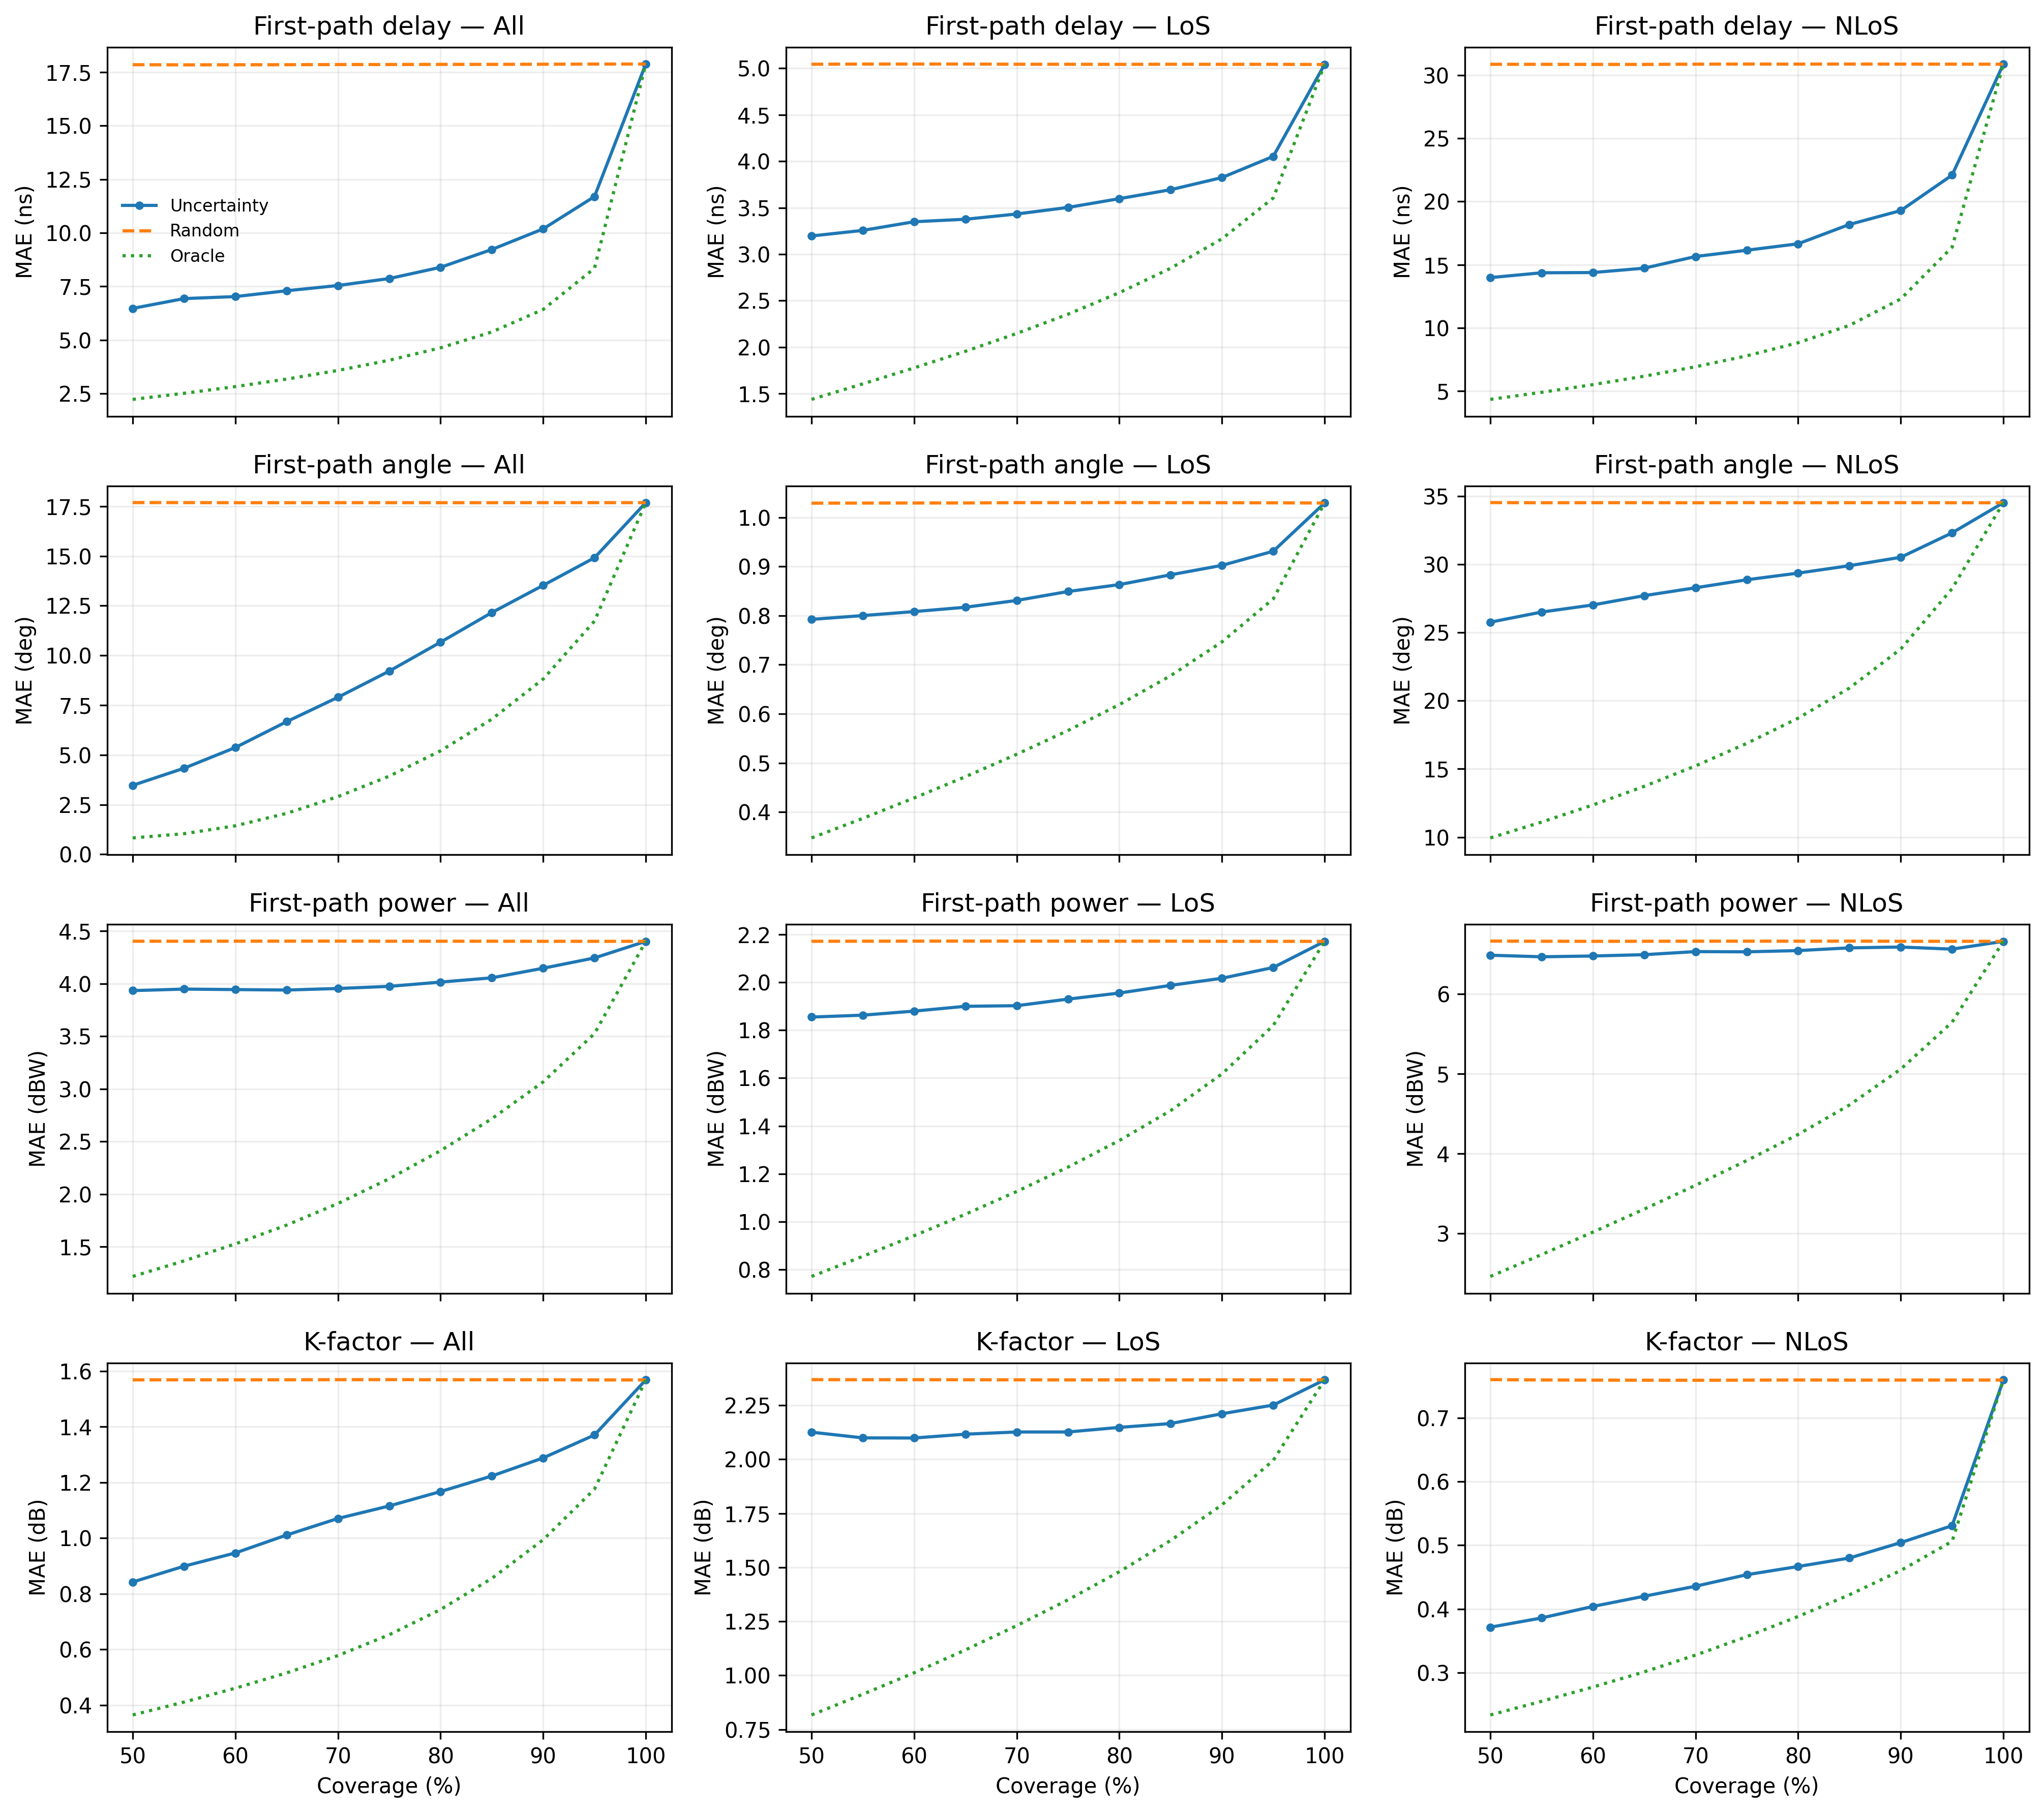
\includegraphics[width=\columnwidth]{figures/risk_coverage_all_metrics.png}
\caption{Risk--coverage curves from the three-seed ensemble for first-path delay, angle, power, and
$K$-factor, evaluated jointly and by LoS/NLoS regime. Blue curves rank samples by ensemble
disagreement, orange lines show random rejection, and green curves give the unattainable oracle
ranking by realized error. Lower coverage means that more high-uncertainty reports are deferred.}
\label{fig:risk-coverage-all}
\end{figure}

Figure~\ref{fig:risk-coverage-all} expands the selective-prediction analysis in
Figure~\ref{fig:nlos-selective-prediction}. Ensemble disagreement is informative for delay and angle:
their MAEs fall steadily as high-uncertainty samples are removed, with the largest absolute benefit in
the NLoS regime. Power is less separable, especially for NLoS, indicating that seed disagreement does
not capture every raw-scale failure. $K$-factor improves more consistently, although its LoS and
NLoS scales differ. The remaining gap to the oracle curves quantifies room for better uncertainty
estimation. These curves support selective deployment rather than replacement of the full-coverage
main metrics: deferred samples require another CSI observation, multi-numerology fusion, or review.

\subsection{Inference Cost}

\begin{table}[t]
\centering
\caption{Physical quality on the inference-cost cohort. Decoder first-delay values can differ from
the learned-baseline table because this benchmark uses a different cohort; model suffixes make this explicit.}
\label{tab:complete-cost}
\scriptsize
\setlength{\tabcolsep}{2.2pt}
\resizebox{\columnwidth}{!}{%
\begin{tabular}{lcccc}
\toprule
\textbf{Method} & \textbf{Delay (ns) $\downarrow$} & \textbf{Angle ($^\circ$) $\downarrow$} &
\textbf{Power (dB) $\downarrow$} & \textbf{$K$ (dB) $\downarrow$} \\
\midrule
\rowcolor{modelblue}\textbf{CSI2TEXT-PGMT-COST-BENCHMARK} & \best{20.68} & $\best{19.55\pm0.38}$ & $5.02\pm0.31$ & $1.87\pm0.24$ \\
\textbf{Single-task} & $47.75\pm5.22$ & $20.65\pm0.32$ & $\best{3.85\pm0.23}$ & $\best{1.42\pm0.04}$ \\
\textbf{PDP/IFFT+MLP} & $27.58\pm5.05$ & $41.62\pm0.68$ & $12.66\pm0.32$ & $5.22\pm0.22$ \\
\textbf{Flattened MLP} & $109.98\pm0.87$ & $34.85\pm0.26$ & $13.06\pm1.17$ & $5.28\pm1.02$ \\
\textbf{Transformer} & $265.91\pm0.02$ & $53.37\pm0.02$ & $38.18\pm0.00$ & $22.52\pm0.00$ \\
\textbf{CNN} & $1619.16\pm1238.13$ & $102.18\pm42.31$ & $14595.56\pm18584.48$ & $55.55\pm34.37$ \\
\textbf{Qwen3-1.7B} & 177.66 & 42.84 & 6.17 & 2.56 \\
\textbf{Qwen3.5-2B} & 162.47 & 42.37 & 5.85 & 2.53 \\
\textbf{DeepSeek-8B} & 232.66 & 59.16 & 27.77 & 16.42 \\
\textbf{InternLM3-8B} & 165.56 & 40.22 & 5.96 & 2.49 \\
\bottomrule
\end{tabular}}
\end{table}

The runtime and memory measurements are consolidated in Table~\ref{tab:inference-cost-main}. Latency is
measured end to end on 200 common examples; quality uses the 1,000-example decoder cohort.
Conventional models use FP32 and direct decoders use 4-bit NF4 weights with BF16
computation. The structured pipeline needs 13.58 ms and 0.13 GB, versus 11--23 s and
1.53--6.18 GB for autoregressive decoders. This is a deployment advantage rather than a replacement
for the physical and text measurements.


For completeness, the original Pareto visualization normalizes each continuous MAE as
\begin{equation}
q_m=\frac{1}{1+\mathrm{MAE}_m/T_m},
\end{equation}
where $T_m$ is the field-specific tolerance. The five shared physical fields are
\[
\mathcal M_A=\{\tau_1,\theta_1,p_1,K,n_{\mathrm{refl}}\}.
\]
For this set,
\begin{equation}
S_{\mathrm{phys}}=100\left(\prod_{m\in\mathcal M_A}q_m\right)^{1/5}.
\end{equation}
For the eight-field continuous set $\mathcal M_C$---first and LoS delay, delay spread, first and LoS
angle, angular spread, first-path power, and $K$ factor---the score is
\begin{equation}
S_{\mathrm{cont}}=100\left(\prod_{m\in\mathcal M_C}q_m\right)^{1/8}.
\end{equation}
The structural and text components are
\begin{align}
S_{\mathrm{struct}}&=100\left(a_{\mathrm{LoS}}a_{\mathrm{path}}a_{\mathrm{refl}}
a_{\mathrm{rpath}}\right)^{1/4},\\
S_{\mathrm{text}}&=100\left(F A_{\mathrm{num}}F_{\mathrm{slot}}(1-H)
A_{\mathrm{delay}}\right)^{1/5},
\end{align}
and the complete score is
\begin{equation}
S_{\mathrm{complete}}=0.50S_{\mathrm{cont}}+0.20S_{\mathrm{struct}}+0.30S_{\mathrm{text}}.
\end{equation}
Here $a_{\mathrm{LoS}}$ averages visibility-state accuracy and macro-F1;
$a_{\mathrm{path}}$ and $a_{\mathrm{rpath}}$ are within-one count accuracies;
$a_{\mathrm{refl}}$ is reflection-bin accuracy; $F$ is factuality; $A_{\mathrm{num}}$ is numerical
tolerance accuracy; $F_{\mathrm{slot}}$ is slot F1; $H$ is hallucination rate; and
$A_{\mathrm{delay}}$ is delay tolerance accuracy. Rule consistency is deliberately excluded.
For CSI2TEXT-PGMT-COST-BENCHMARK, the original visualization gives
$S_{\mathrm{complete}}=78.28\pm0.23$, including
$S_{\mathrm{struct}}=87.34\pm0.18$ and $S_{\mathrm{text}}=94.53\pm0.19$.
Geometric means penalize a single failed field, but the tolerances and the 0.50/0.20/0.30 weights are
design choices that can change rankings. The composite is therefore a visualization aid, not a
replacement for the raw measurements.

\subsection{Reflected-Path Extension}

The main record predicts total reflection-interaction count. A separate head extends the record with
the number of distinct reflected paths. The extension uses RPATH-100K, a naturally imbalanced
100,000-example cohort containing 13,628 LoS and 86,372 NLoS links. Its 80,000/20,000 split contains
10,902/69,098 LoS/NLoS training examples and 2,726/17,274 test examples, so it is not pooled with
the balanced main comparison.

The verbalized reflected-path count reaches MAE $0.091\pm0.007$, RMSE $0.234\pm0.008$, and
within-one accuracy $98.82\pm0.06\%$. Complete descriptions reach
$94.06\pm1.07\%$ factuality, $99.974\pm0.012\%$ numeric-slot F1,
$0.0437\pm0.0200\%$ hallucination, $70.63\pm5.48\%$ numerical tolerance accuracy, and
$99.872\pm0.029\%$ rule consistency. The result demonstrates that total reflection multiplicity and
the number of reflection-bearing paths can be modeled separately. Its strong NLoS skew precludes a
direct numerical comparison with the balanced main cohort.

\section{Qualitative Results, Failure Cases, and Limitations}

\subsection{Representative Channel-Report Templates}

The deterministic verbalizer maps each corrected field to one auditable sentence slot. A LoS report
contains the predicted environment and visibility state, retained path count, first-path delay, angle and
power, delay and angular spreads, $K$ factor, LoS-specific delay and angle, total reflection-interaction
count, and reflected-path count when the extension is enabled. An NLoS report suppresses LoS-only
slots. The corresponding templates are
\begin{align*}
\text{LoS: }&[e,\mathrm{LoS},n_p,\tau_1,\theta_1,p_1,\sigma_\tau,\sigma_\theta,\\[-2pt]
&\qquad K,\tau_{\mathrm{LoS}},\theta_{\mathrm{LoS}},n_{\mathrm{refl}},n_{\mathrm{rpath}}],\\
\text{NLoS: }&[e,\mathrm{NLoS},n_p,\tau_1,\theta_1,p_1,\sigma_\tau,\sigma_\theta,\\[-2pt]
&\qquad K,n_{\mathrm{refl}},n_{\mathrm{rpath}}].
\end{align*}
Qualitative inspection compares every emitted number with the corresponding corrected field rather
than judging surface fluency alone. A reproducible case audit records the sample and cohort ID,
reference record, pre-correction prediction, corrected record, final description, and field-level error.

\subsection{Structured Model Versus Direct Decoder Audits}

The direct decoders usually master the output schema: their slot F1 values are close to those of the
structured model. Their main failure is numerical grounding, especially delay. A useful qualitative
comparison must therefore mark separately: missing slots, unsupported slots, internally inconsistent
values, and values that are syntactically valid but outside physical tolerance. This distinction prevents
perfect rule consistency from being misread as perfect channel prediction.

\subsection{Before and After Relational Correction}

Relational correction operates only on the emitted record. For predicted LoS samples, the earliest-path
and direct-LoS delays are reconciled to the dedicated LoS-delay estimate; negative spreads and invalid
counts are clamped; and at least one retained path is enforced. The raw head outputs remain the proper
measure of neural prediction quality. Before/after examples should therefore display both records and
identify which fields were changed by deterministic rules.

\subsection{LoS and NLoS Failure Cases}

The dominant failure regime is NLoS first-path inference. Direct-path geometry produces stable delay
and angular signatures, while an indirect first retained path is more weakly constrained by the supplied
transmitter-side observation. Failure analysis should be stratified into: incorrect first-path delay,
incorrect receiver-side angle, absolute-power error, reflection-count error, and schema-level error.
The main results show that schema errors are rare relative to physical estimation errors. Future
qualitative panels should sample both typical and high-error cases from fixed cohort IDs rather than
selecting only visually favorable outputs.

\subsection{Scope and Limitations}

All labels and physical relations are derived from finite ray-tracing exports. They inherit the
simulator's path-retention policy, fixed transmit-power assumption, maximum retained-path count, and
reflection encoding. The work establishes a controlled simulator-grounded interface, not field
deployment. Measured-channel validation remains necessary.

The language layer demonstrates auditable realization of a typed record rather than unrestricted
conversation or stylistic generation. Composite factuality is slot based and tolerance dependent; raw
per-field errors must remain visible. Generalization covers selected frequency and array shifts, not
arbitrary bandwidths, carriers, calibration errors, non-Gaussian interference, or hardware
impairments. The AWGN experiment probes one controlled corruption axis only.

The direct decoders have one run each and are not parameter matched, so small ranking differences
are unresolved. Multi-task sharing and language alignment do not improve every target. The robust
conclusion is narrower: target-appropriate representations and structured prediction ground reports
better than direct decoding, while NLoS multipath recovery remains the principal limitation.
